\section{UIProtocol}
This chapter introduces the reader to the UIProtocol, its architecture and communication between UIP client and server.

\subsection{About UIProtocol}
Universal Interface Protocol (UIProtocol, UIP) is a user interface specification language \cite{uip} being developed at FEE CTU for research purposes. At the time of writing, the specification is not publicly available. UIProtocol provides means for describing user interfaces and transferring data related to interaction between user and an UIProtocol based application. It is designed to be cross-platform, programming language independent and easily localized \cite{uip}.

The goal of UIProtocol is to simplify development for various target platforms: with UIProtocol, a developer only has to describe the application once, and the application then runs on all platforms with UIP client implementation. This should simplify the development process and make one application easily available to multiple platforms. UIProtocol client uses platform-native UI components, which makes it different from HTML-based applications.

UIProtocol is an application protocol that allows for describing the hierarchical structure of GUIs along with the placement and visual appearance of the containers and components. It is designed for a client-server system and for facilitating client-server applications it defines the communication rules between the two. The communication is based on exchange of XML (or other supported) documents. The client first initiates the communication and receives a UI description document from the server.

The description can be of two different types: interfaces, i.e. the UI components and containers, and models which contain the data displayed in the UI components. The communication from client to server only consists of event descriptions, that is, actions that the user has done (e.g. a button click). The architecture of UIProtocol is shown in figure \ref{fig:UIParchitecture} which also indicates the information flow between the client and server. The figure also shows Actions, which are an advanced, optional feature and we will not cover it.

\begin{figure}[ht!]
\centering
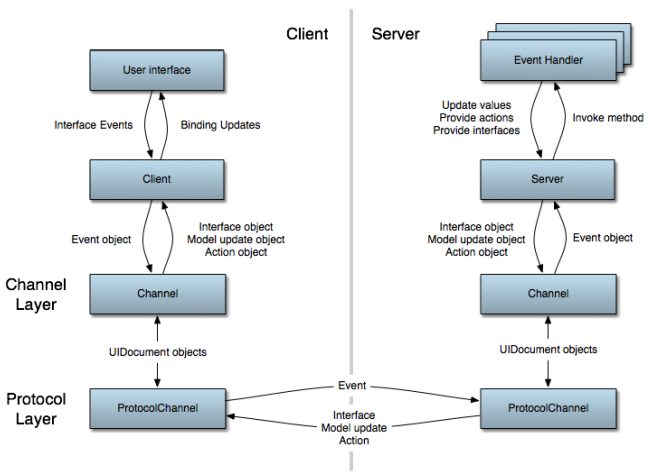
\includegraphics[width=135mm]{pics/UIParchitecture.png}
\caption{the client-server architecture of UIP, taken from \cite{uip}}

\label{fig:UIParchitecture}
\end{figure}
\noindent
Let us give an example of when an event is sent to the server: Consider a situation when a user requests a weather app to his device. As he enters his location and presses a button to request the weather information, part of the job is done directly by the client and the other part is sent to the server. The part done directly at the client are easy tasks, such as visual effects when pressing the button. The request for weather information is then sent to the server. Server processes the request and responds by sending the interface structure information, UI components' description and the weather data. This is displayed to the user, who then has other options to interact with the app.

The documents of UIProtocol can be sent in either direction usually through a single channel without waiting for a request, i.e. the server can send updates to the client as soon as the displayed information needs to be updated, without waiting for an update request.

Should there be such need, there is the possibility of both client and server running on the same machine although this is not a typical usage.

\subsubsection{UIProtocol Client}
UIProtocol client is thin, i.e. no application code is executed on the client side \cite{uip}. The device running the client is thought to be the one user directly interacts with, that is, it renders the content to the user and receives input from her. From the UIProtocol point of view, the client device is also considered insecure, i.e. the device may be misused to send invalid data to the server and may be used to attack it.

The UIP client may not implement the whole feature set defined by UIProtocol \cite{uip}. What has to be implemented is the minimal functionality, i.e. a client that is able to render user interfaces, send event information to the server and update the application by data coming from it. A use case diagram of actions performed by user in the client app is shown in figure \ref{fig:UIPusecase}.

\subsubsection{UIProtocol Server}
UIProtocol server is the part of the architecture which is responsible for evaluating the client events and sending a correct response - this is where the application logic is executed \cite{uip}. Server must be able to service multiple clients simultaneously and is intended to run on a machine which is considered safe \cite{uip}. A use case diagram of server actions is shown in figure \ref{fig:UIPusecase}.

\begin{figure}[ht!]
\centering
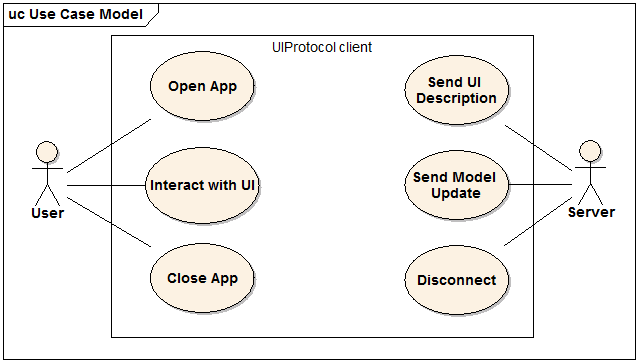
\includegraphics[width=120mm]{pics/usecase.png}
\caption{Use case diagram for user and server}

\label{fig:UIPusecase}
\end{figure}

\subsection{Syntax of UIProtocol}
The UIP document syntax in listing \ref{uipSyntax} shows the four possible tags and the root element, with the actions tag being optional. The tags define the behavior of the application and are covered later in the chapter, with the exception of the actions tag.

Every UIProtocol document must contain an XML header with the version and encoding (UTF-8 recommended).

\lstinputlisting[label=uipSyntax,caption=UIP document Syntax]{sources/uipSyntax.xml}



\subsection{Elements of UIProtocol Communication}
As mentioned previously, the information exchange between client and server concerns interfaces and models (which are sent from server to client) and events (sent from client to server). In the following subsections we will describe these in greater detail and also include more information on UIProtocol syntax.

\subsubsection{Interfaces}
Interface describes the structure and components of the user interface. Every interface can nest containers and elements that form a part of user interface. An example can be seen in listing \ref{uipInterface}. The listing includes containers and elements of different types, for example \texttt{public.input.text} is a standard component which will be rendered as an UI control into which the user can enter text. It also shows how one interface can be embedded into other. This is done by an element or container with class name corresponding to different interface's class.

The interfaces are uniquely identified by the class attribute (unlike most other objects in UIProtocol and other markup languages identified by id attribute).

\lstinputlisting[label=uipInterface,caption=Interface Description Example]{sources/interfaces.xml}
%todo containers and elements - and the classes of elements

\subsubsection{Events}
Events inform the server that some action was triggered at the client side (e.g. a button press) or that there was some other update (e.g. change in sensor readings). This is the mechanism of client-to-server communication and therefore has to be supported by the client. The event element contains a unique id which specifies the event source. An event can contain any number of properties which describe it in greater detail. An example is shown in listing \ref{uipEvents}.
\lstinputlisting[label=uipEvents,caption=Events Example]{sources/uipEvents.xml}

\paragraph{Properties}
\label{subsec:props}
Properties are the most nested elements of UIP documents and define the visual appearance of UI controls, their positioning, content and much more. They are heavily used in many UIP's structures - in Models, in styling and more. Every property has to have a name, which defines what feature of the connected object the property describes. For example, the property in listing \ref{uipInterface} with name \texttt{text} defines the text displayed in the text field. Value is a constant that will define the text.

The mentioned property can also contain a key attribute which, if set, binds the displayed value to a model property (see the next paragraph).
%The part before the colon references a model and the part after colon references a property within the model. That is, if there is a model \texttt{gui} with property \texttt{fstName}, value of \texttt{fstName} property is used. Moreover, whenever the value of the \texttt{fstName} property is updated by the server, the update is automatically reflected in all bound properties.

\lstinputlisting[label=uipProperty,caption=Property key example]{sources/uipProperty.xml}

\subsubsection{Models and Model Binding}
\label{subsec:models}
Models serve as a storage for data. Within models, data is stored in properties which are uniquely identified by model name and name of the property within that model. As explained in the previous paragraph, properties can be used to define content and appearance of UI elements and more. The property value can be provided as a constant, or it can refer to a model, using the key. The key is separated by colon into two parts - the first referencing a model and the second referencing a property within the model (see listing \ref{uipProperty} for an example).

For example, consider the element in listing \ref{uipProperty}. The property representing the UI control's text contains a nonempty key. It follows that the \texttt{modelName} model is requested from the server. Upon its arrival, the \texttt{modelPropertyName} property is looked up in the model and the text of the UI control is set to this UIP property's value. Also, a data binding between the \texttt{modelPropertyName} property and the UI element's text property is created so that when the client receives an update of the \texttt{modelPropertyName} property, the UI element's text gets immediately updated.

When updating the value of a model property, all UI elements bound to the model property are updated. For example, there may be two representations of humidity level in a given environment (text and a graphical representation). If they are both bound to the same model property, update of the given property will be immediately reflected by both.

Note that Models in UIP are application-wide so they can be referred to from any point of the application.

\endinput